\section{Hardware}
\label{sec:chapterexample}

Das System wird Hardwareseitig in zwei Teile unterteilt. Der Server, die zentrale Einheit und die Aussensprechstelle. An beide Orte wird eine Raspberry Pi 3 und das nötige Hardware eingesetzt.

\subsection{Server}
\label{sec:chapterexample}

Der Server wird mit einem Relay-Board verbunden. Diese wird die Gongs und die Türöffner bedienen. An dieser Stelle ist die Hardware-Konfiguration sehr einfach. Je nach wie viele Gongs und Türe verbunden werden müssen, könnten bis zwei 8-Channel Relayboards verbunden werden.
\\

<-- ABBILDUNG CON LA PI E I RELAY E I PIN A CUI SONO COLLEGATI
\\
\\

\subsection{Aussensprechstelle}
\label{sec:chapterexample}

Bei der Aussensprechstelle wird auch eine Raspberry Pi eingesetzt. Hier sind mehrere Zusatzkomponenten notwendig. Die Speisung an dieser stelle erfolgt nur über PoE, aus diesem Grund ist PoE-Splitter vorhanden.
\\
\\
Für die Audiowiedergabe ist ein kleines Lautsprecher und ein Verstärker nötig. Die Chinch-Anschluss der Raspberry Pi hat eine zu kleine innere Widerstand um direkt ein solches Lautsprecher anschliessen zu können. Die Hauptproblematik nun besteht darin, dass die Massen des Raspberry Pi, der Verstärker und des Audio-Interface alle zusammen gekoppelt sind. Das führt zu Brunschleifen die wiederum Störsignale auf dem Audio-Ausgang erzeugen. Um das zu vermeiden ist eine Massentrennfilter an dieser Stelle notwendig.
\\

<-- ABBILDUNG CON LA PI E COMPONENTI COLLEGATI
\\
\\

\subsection{PoE}
\label{sec:poe}
Moderne Hausalte werden meistens mit ethernet Verkabelung verlegt. Ziel des Aussensprechstelle ist die Installationskosten zu senken und die Montage zu vereinfachen. Drei Anschlusse werden von den Aussensprechstelle benötigt um sein Ziel zu erreichen und zwar Strom, Internetverbindung und eine Leitung der für den Türöffner zuständig ist. Alle diese Fünktionalität können in einem Kat 7 Ethernet Kabel zusammengeführt werden. 
\\
Cisco Catalyst 3560g welcher für den PoE Stromversorgung zuständigt ist verwendet das Phantomspeisung oder Mode A. Das heisst dass die mit Datenübertragung belegten Adern mit der Stromversorgung überlagert werden. Diese ist möglich da Elektrizität hat eine niedrige Frequenz von 60 Hz und Datenübertragungen im bereich 10-100MHz liegt.

\begin{figure}[htb!]
	\begin{center}
		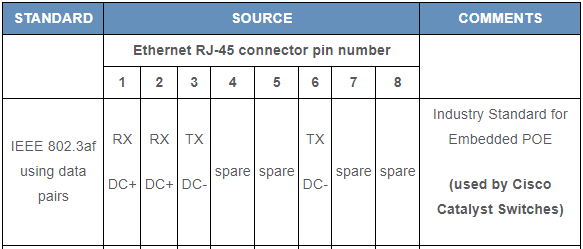
\includegraphics[width=0.89\textwidth]{CatalystPoEpinouts}
		\caption[Catalyst 3560g PoE Pinbelegung]{Catalyst Pinouts}
		\label{fig:catalystPinouts}
	\end{center}
\end{figure}


Die einzige Nachteil bei dieser Konfiguration 

<-- ABBILDUNG CON IL CAVO ETHERNET
\\


\newpage